\documentclass[12pt,aspectratio=169]{beamer}
\usepackage{unito}

\usepackage{booktabs}
\usepackage[export]{adjustbox}

% TODO:
% - Aggiungere slide positive/negative (immagine SupCON)
% - Enfasi su fenotipi. Sono importanti perché se c'è correlazione tra anatomia
% e fenotipi è possibile scoprire dei biomarker (una ROI specifica può essere
% relazionato ad un fenotipo)
% - Migliorare discorso su slide "Results". Parti prima da tabella e poi al polar (enfasi su schizconnect).
% - Spiegare i task migliori sulla seconda slide results (e quale metrica). Due parole sul fatto che è "novel" 
% - Opzionale: Provare a modificare Contrastive Learning
% - Aggiungere delle slides come sezione "Appendice"

% - Bisogna dare un obiettivo preciso iniziale per dare contesto
% - Inverti slide 7 e 8 (non parlare di self-supervised in slide 6)
% - Local/Global descriptor -> Proposed method
% - Migliorare 15 mettendo immagine 12
% - Calcare su molti esperimenti, molti dataset, citare che sono state usate risorse CINECA
% Obiettivo -> Metodo -> (Tanti) Esperimenti -> Risultati -> Sviluppi futuri
% Commenti minori:
% - Mettere reference dei metodi
% - Slide 19 evidenziare i risultati migliori
% - Slide 20 rispetto alle altre baseline

\newcommand{\result}[2]{#1$_{\pm #2}$}

\title{Integrating Anatomical Information in\\Weakly Contrastive Learning for\\ Neuroimaging}
\author{Matteo Brunello}
\supervisor{Marco Grangetto}
\cosupervisor{Carlo Alberto Barbano}

\begin{document}

\maketitle

% \begin{frame}{Neuroimaging}
% \begin{columns}
% \begin{column}{0.6\textwidth}
%     \begin{itemize}
%         \item Broad application in diagnosis and studies related to different neurological disorders
%         \item Different \textbf{acquisition methods} (sMRI, fMRI, dMRI, PET, etc.) to measure different features
%         \item Output of MRI are 3D volumes representing the selected anatomical measure 
%     \end{itemize}
% \end{column}
% \begin{column}{0.4\textwidth}
%     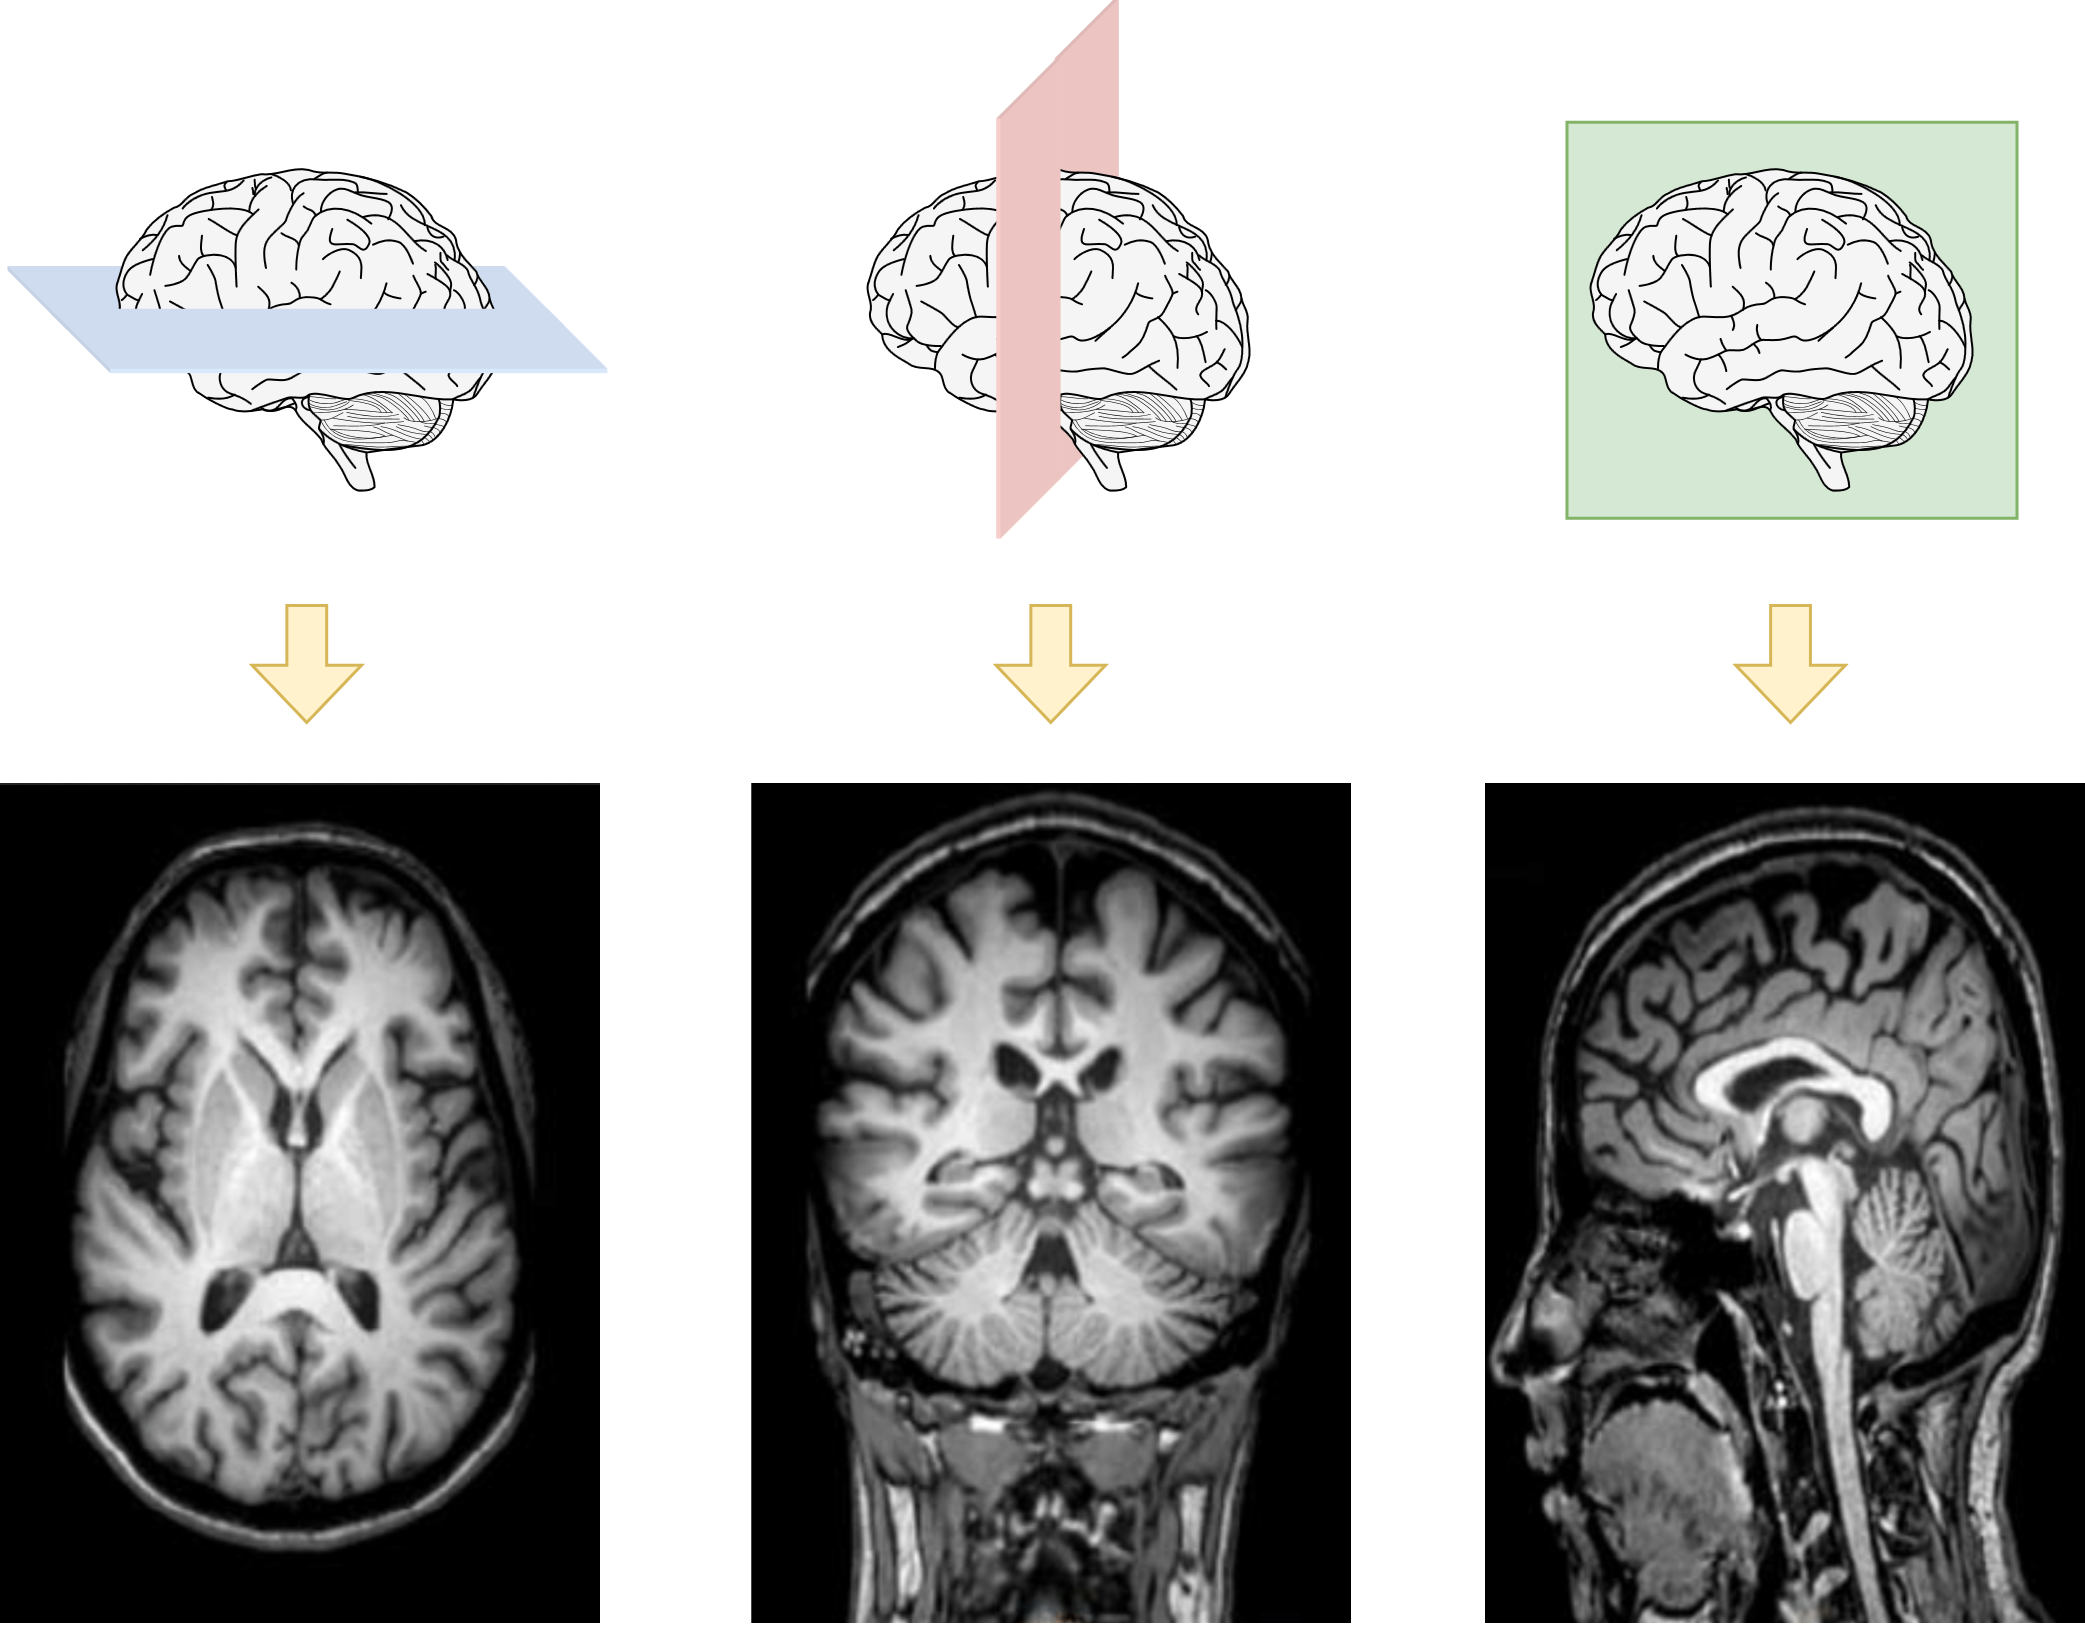
\includegraphics[width=\textwidth]{source/acquisition_planes.png}\\
% \end{column}
% \end{columns}
% \end{frame}

% 1
% \begin{frame}{Deep Learning}
% \begin{itemize}
%     \item Deep learning models are able to \textbf{learn} subtle statistical
%     correlations using a \textbf{large} set of data samples
%     \item Convolutional Neural Networks (CNN) are deep learning models
%     specialized in processing \textbf{image data} as inputs
%     \item They learn to map high dimensional inputs (images) to a
%     low-dimensional vector space called \textbf{latent space}, which captures the
%     essential features in the input data 
% \end{itemize}
% \end{frame}

% % 2
% \begin{frame}{Convolutional Neural Networks}
%     \begin{picture}(0,120)
%     \put(30,0){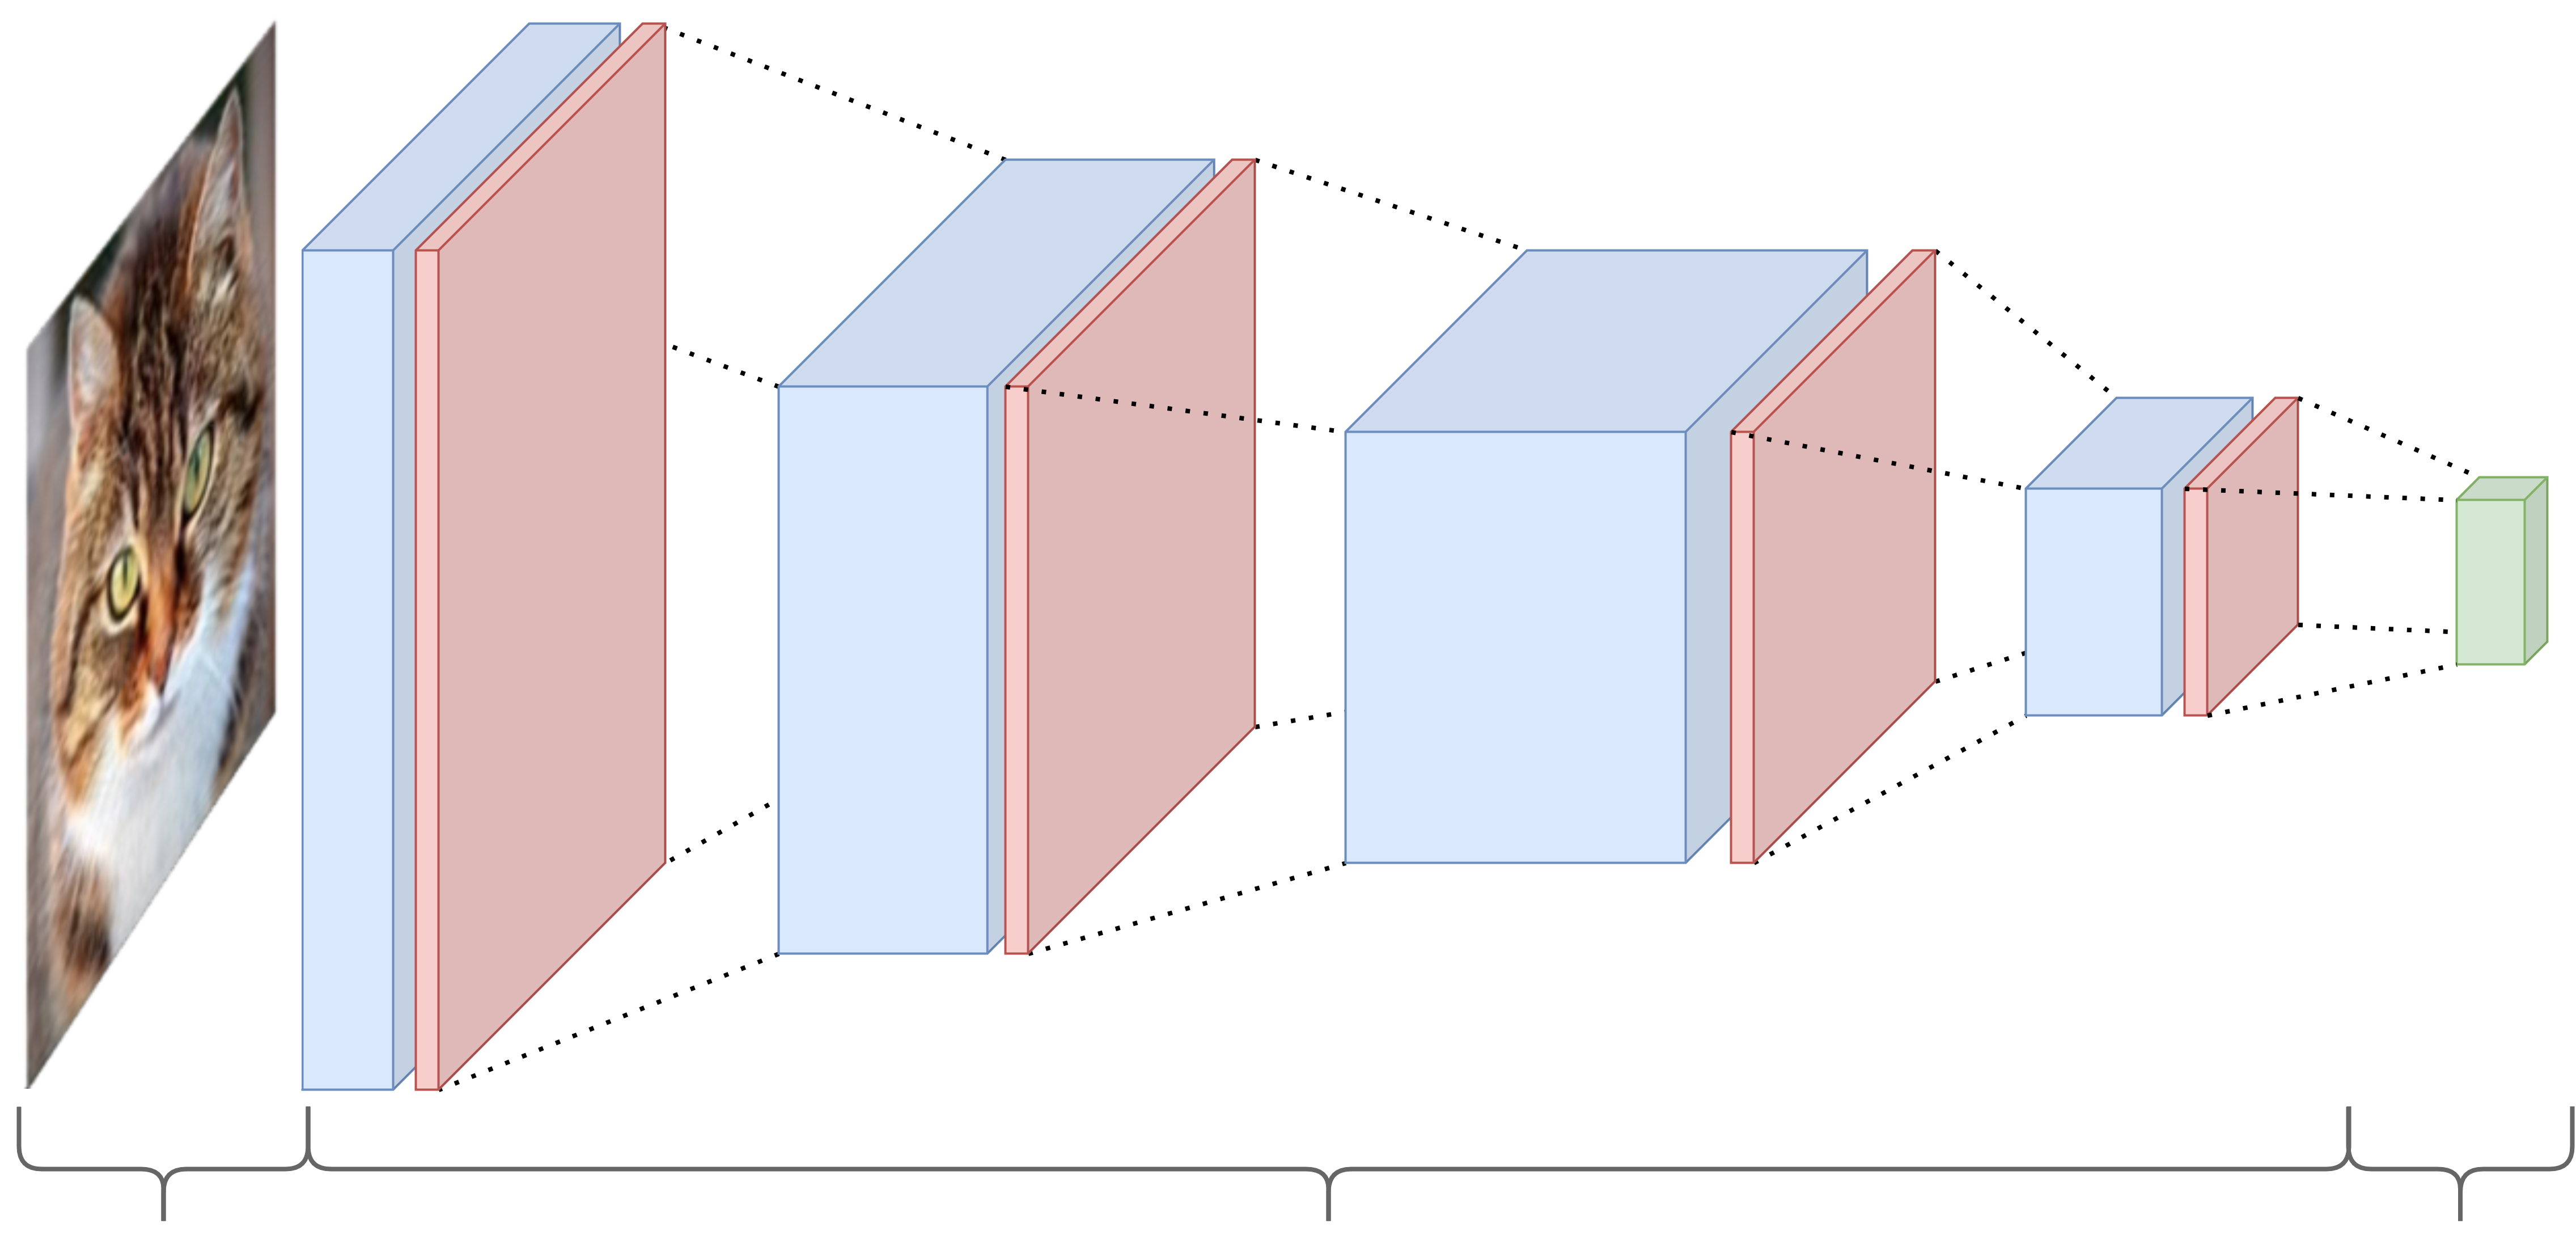
\includegraphics[width=.8\textwidth]{source/convolutional_network.png}}
%     \put(20, -15){Input Image}
%     \put(150, -15){Feature Extractor}
%     \put(280, -15){Embedding Vector}
%     \end{picture}
% \end{frame}

% 3
\begin{frame}{Deep Learning in Neuroimaging}
\begin{itemize}
    \item Deep learning has demonstrated remarkable results across various
    fields that benefit from \textbf{automated image analysis}, including neuroimaging
    \item Neuroimaging concerns the acquisition and analysis of \textbf{brain images}
    \item Neurobiological characterization of psychiatric and neurological
    disorders encompasses clinical, biological and environmental factors
    \item \textbf{Limited} relative size of neuroimaging datasets, especially related to
    specific neurological conditions 
\end{itemize}
\end{frame}

% 4
\begin{frame}{Transfer Learning}
    \begin{picture}(0,0)
    \put(35, -80){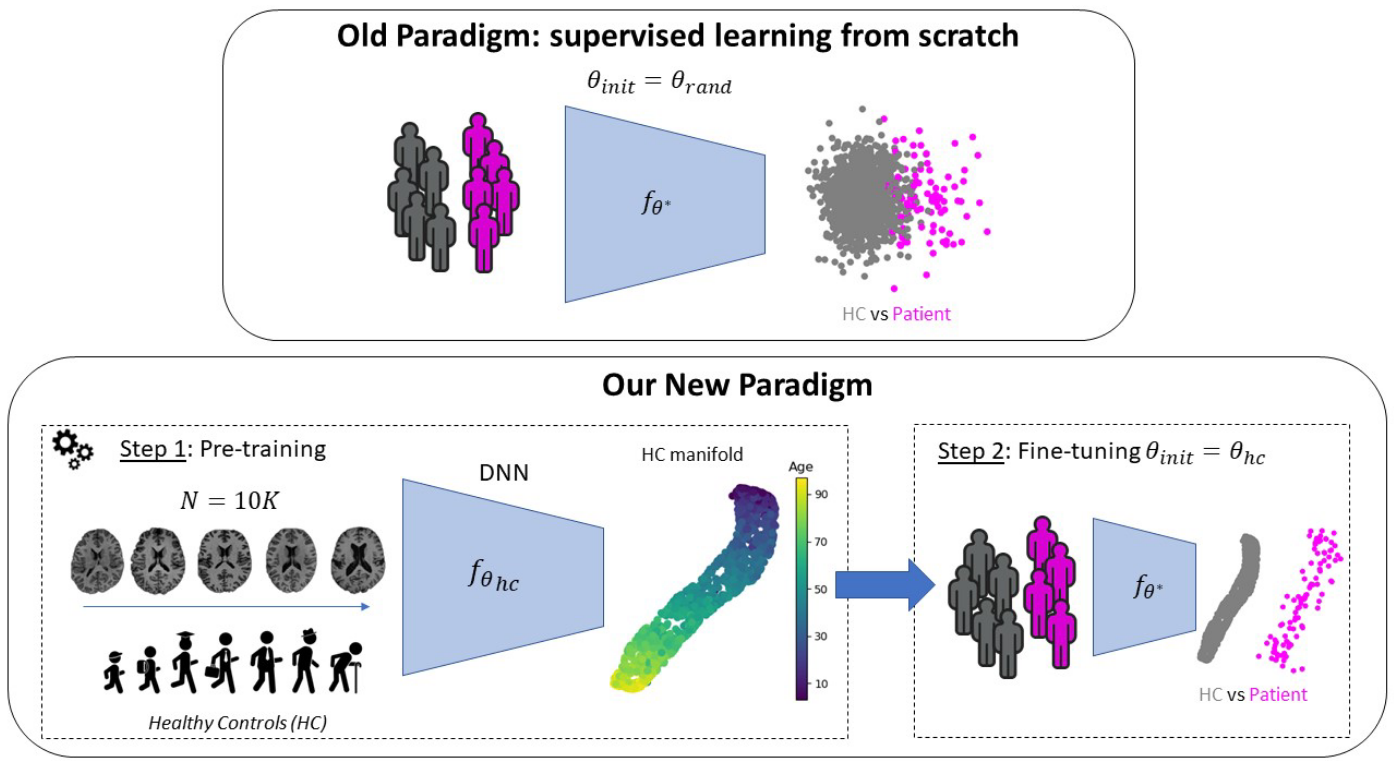
\includegraphics[width=.8\textwidth]{source/transfer_learning.png}}
    \put(125, -95){\small\emph{Credits: Dufumier et. al, 2024}}
    \end{picture}
\end{frame}

\begin{frame}{Contrastive Learning}
\begin{columns}
\begin{column}{0.5\textwidth}
    \begin{itemize}
        \item \textbf{Minimize} the distance between positive pairs of embeddings 
        \item \textbf{Maximize} the distance between negative pairs of embeddings
    \end{itemize}
    \vspace{35pt}
    \begin{equation*}
    \mathscr{L}_{i, j} = - \log \left(
        \frac
        {\exp(s_{i,j} / \tau)}
        {\sum\limits_{a \in A(i)} \exp(s_{i, a} / \tau)}
    \right)
    \end{equation*}
\end{column}
\begin{column}{0.5\textwidth}
\begin{center}
    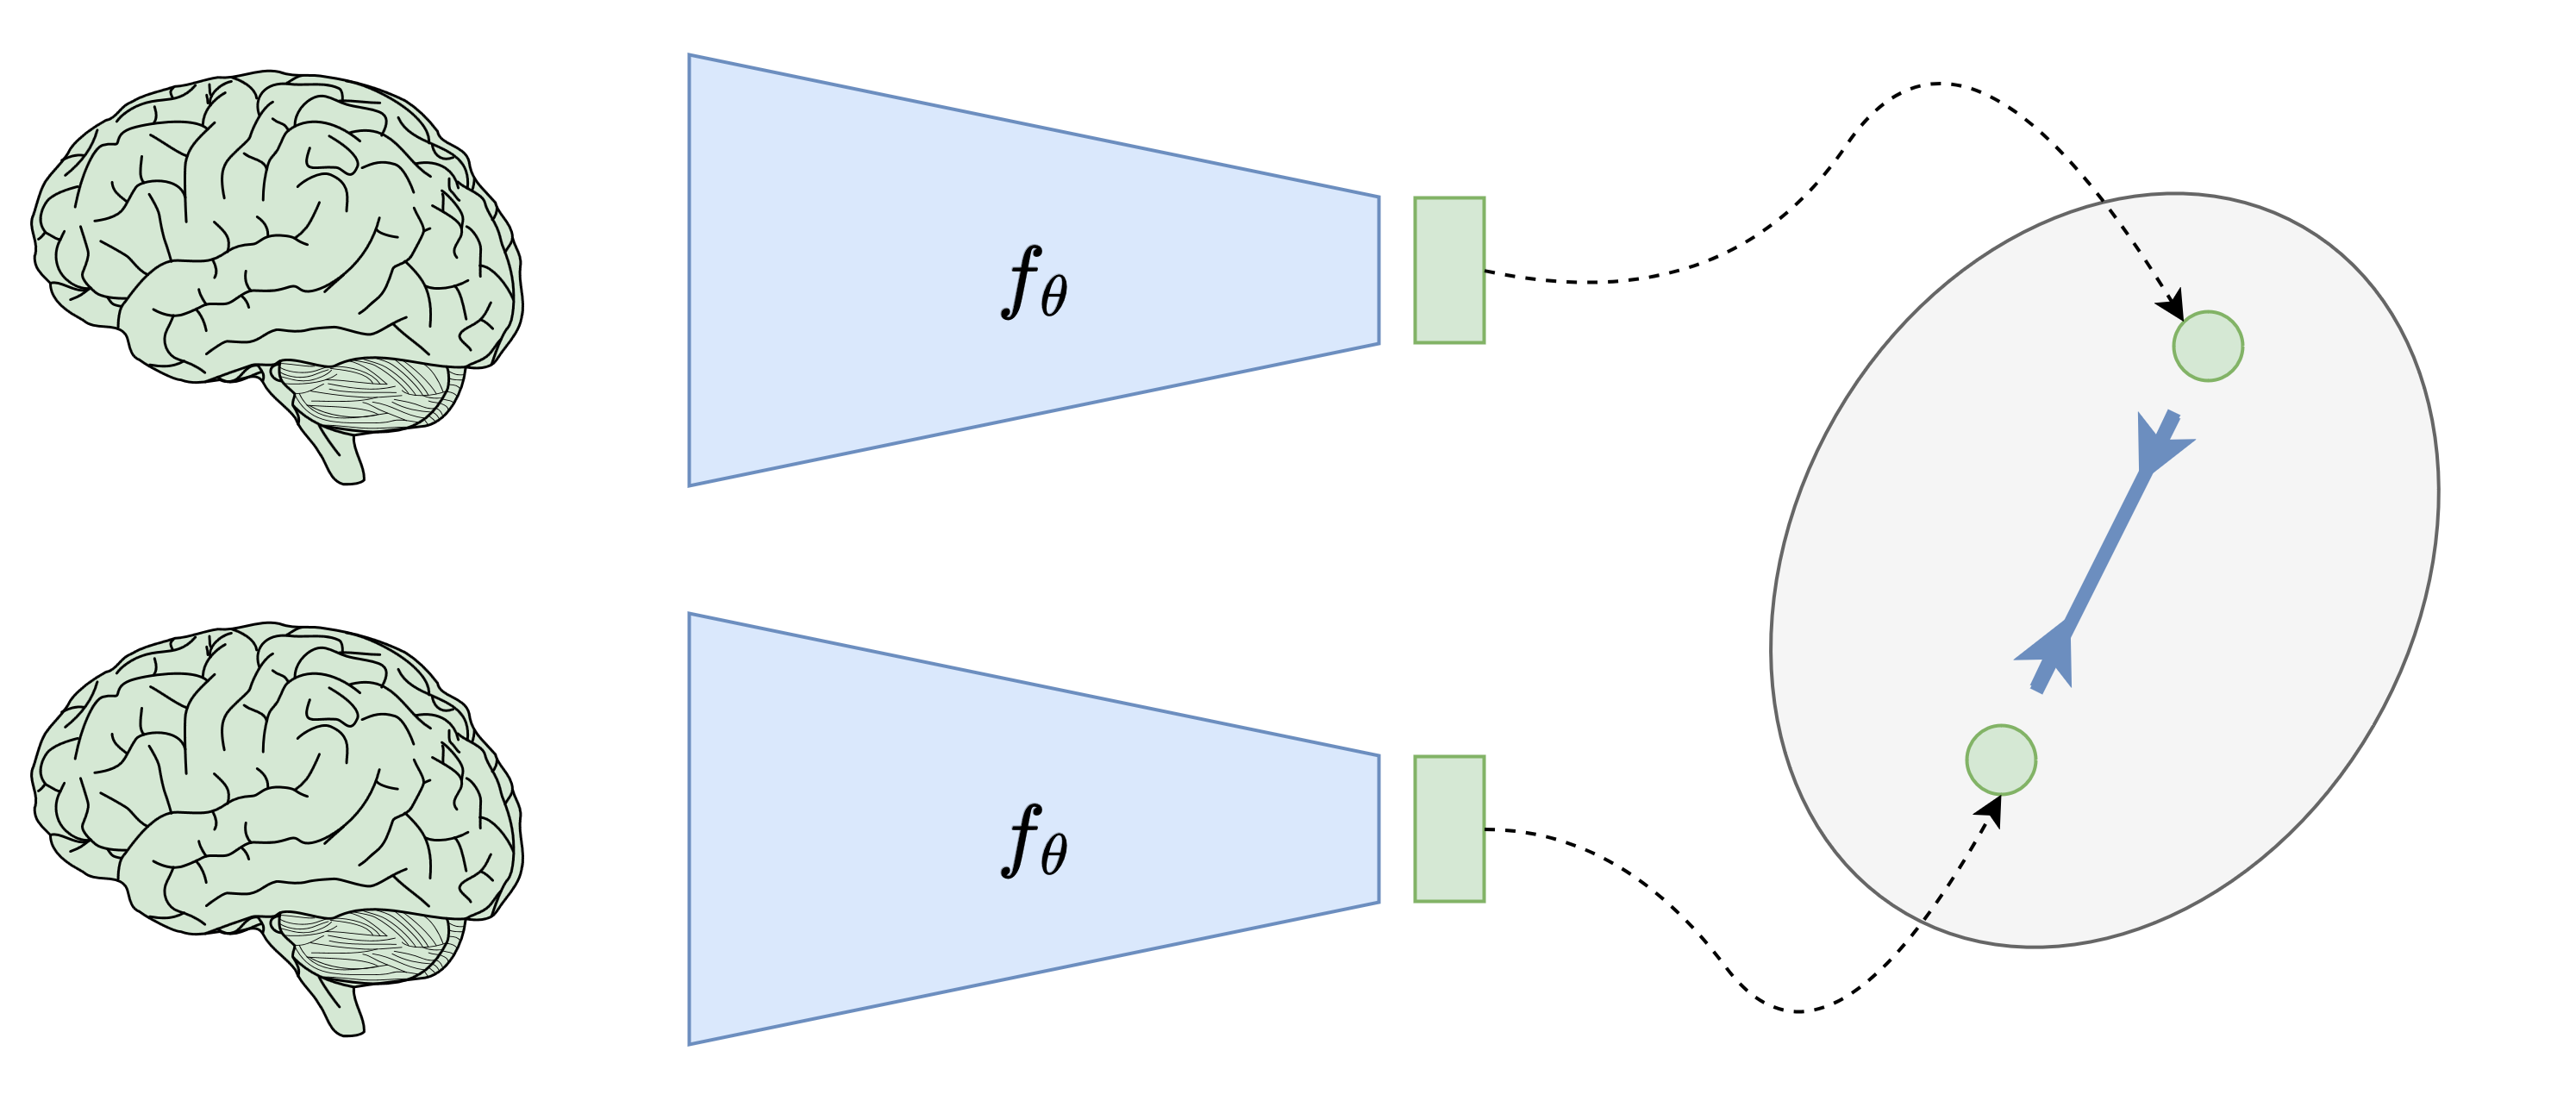
\includegraphics[width=.9\textwidth]{source/contrastive_pulling.png}\\
    \vspace{15pt}
    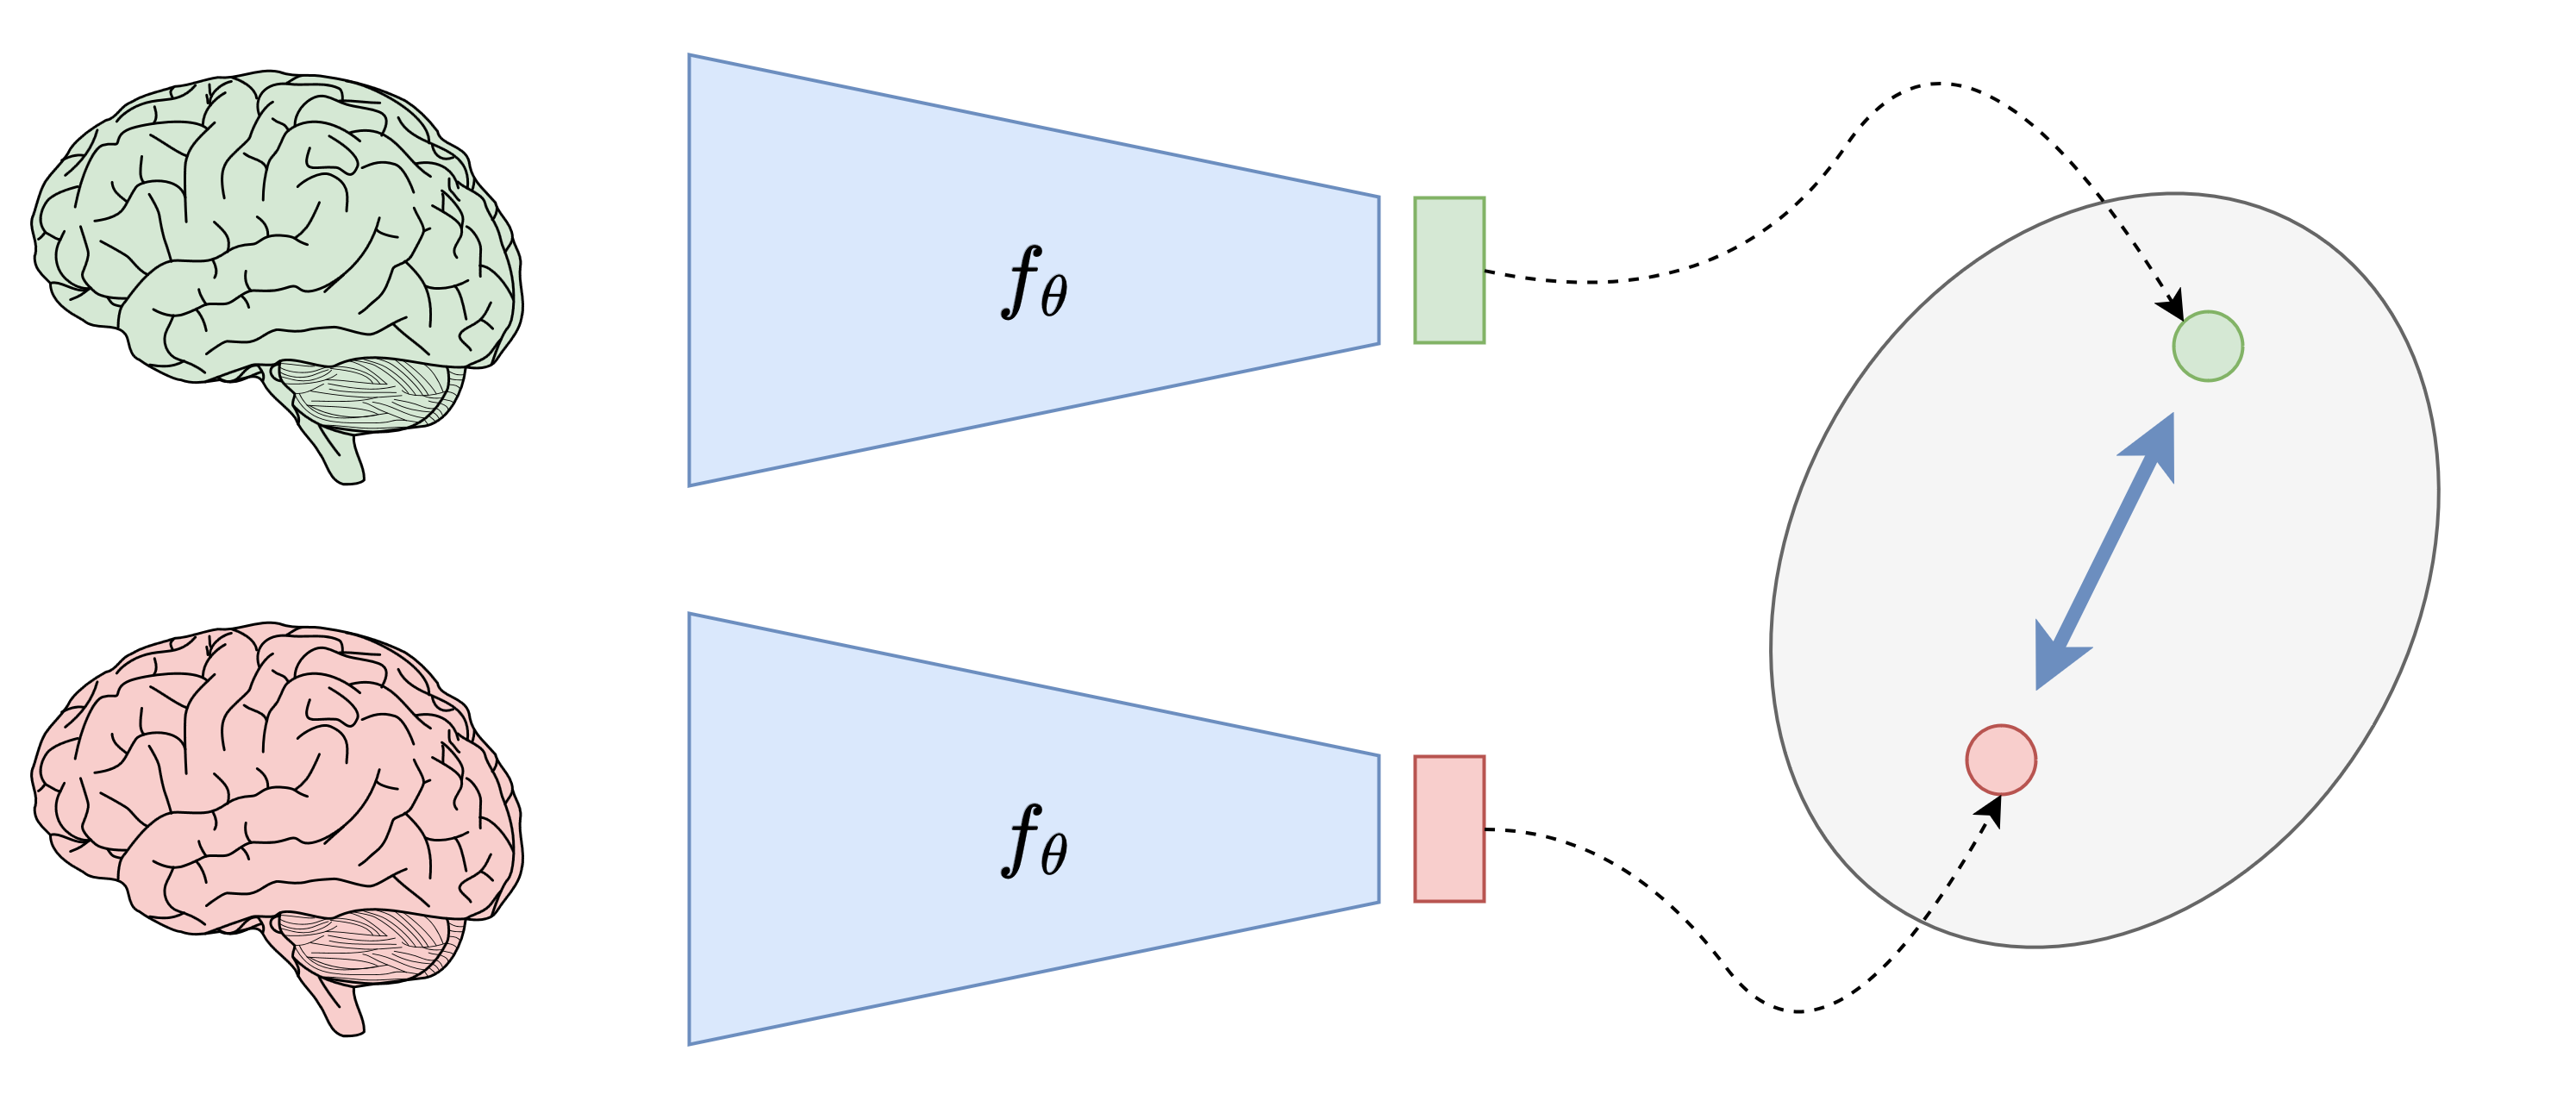
\includegraphics[width=.9\textwidth]{source/contrastive_pushing.png}\\
\end{center}
\end{column}
\end{columns}
\end{frame}

% 7
\begin{frame}{Weakly Supervised Contrastive Learning}
\begin{itemize}
    \item Existing weakly contrastive learning methods augment the learning
    process with the \textbf{age attribute}
    \item These methods works by computing a \textbf{weight term} that increase
    the pushing/pulling strength between latent representations based on the
    closeness of the age attribute
\end{itemize}
\begin{equation*}
    \mathcal{L}^{\text{y-aware}} = 
    -\sum_{k \in A(i)} \frac{w_k}{\sum_t w_t} log
    \left(
    \frac
    {\exp(s_k / \tau)}
    {\sum\limits_{a \in A(i)} \exp(s_a / \tau)}
    \right)
\end{equation*}
Where:
\begin{equation*}
    w_k = K_\sigma(y_i - y_k)
\end{equation*}
\end{frame}

% 8
\begin{frame}{Weakly Supervised Contrastive Learning}
\begin{center}
    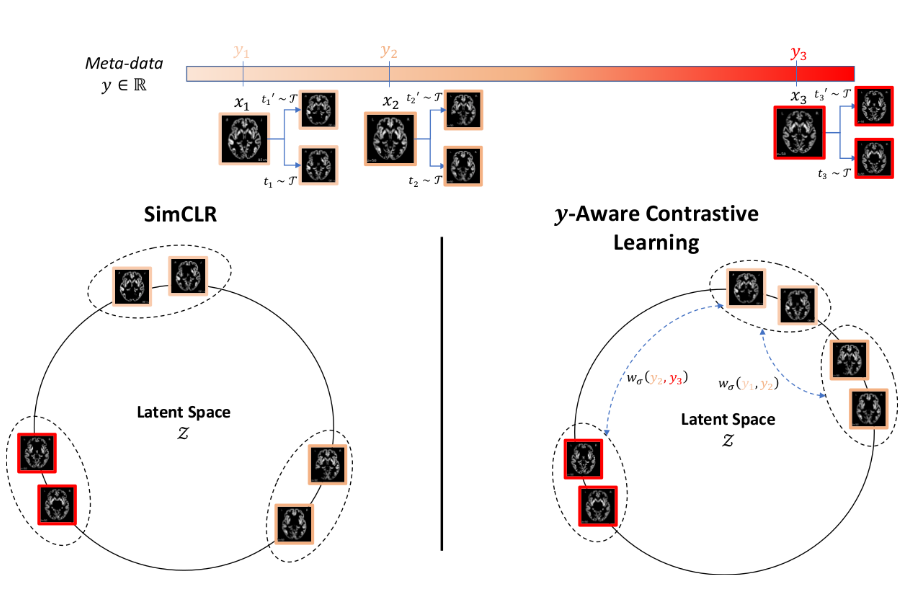
\includegraphics[width=.7\textwidth]{source/yaware.png}\\
\end{center}
\end{frame}

\begin{frame}{Goal of this Thesis}



\begin{columns}
    \begin{column}{.6\textwidth}
        
\begin{itemize}
    \item Neuroimaging datasets commonly include other \textbf{anatomical
    measures} along with \textbf{patient-specific informations} (age, sex, etc.)
    \item Leverage this data during the \textbf{pre-training} process to further
    enhance the learned representations
    \item This may in turn enhance the performance and \textbf{generalizability}
    of the model in various downstream tasks\\ 
\end{itemize}
    \end{column}
    \begin{column}{.4\textwidth}
        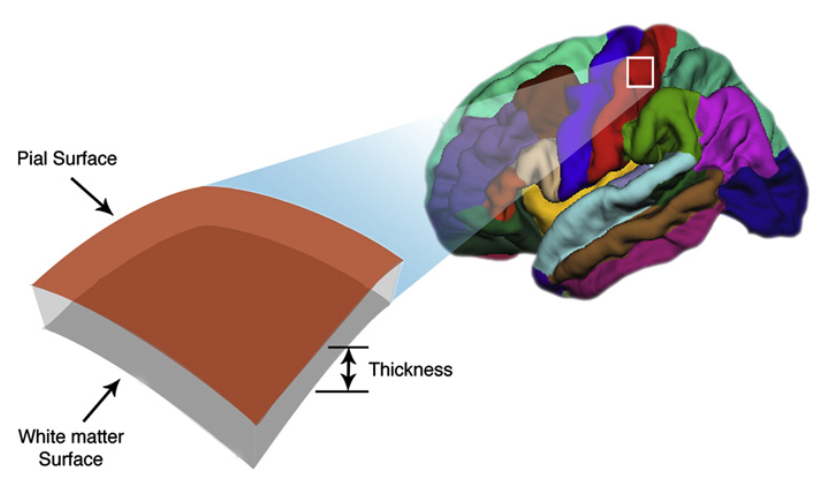
\includegraphics[width=\textwidth]{source/anatomical_measures.png}
    \end{column}
\end{columns}

\end{frame}

\begin{frame}{Current Approach}
    \centering
    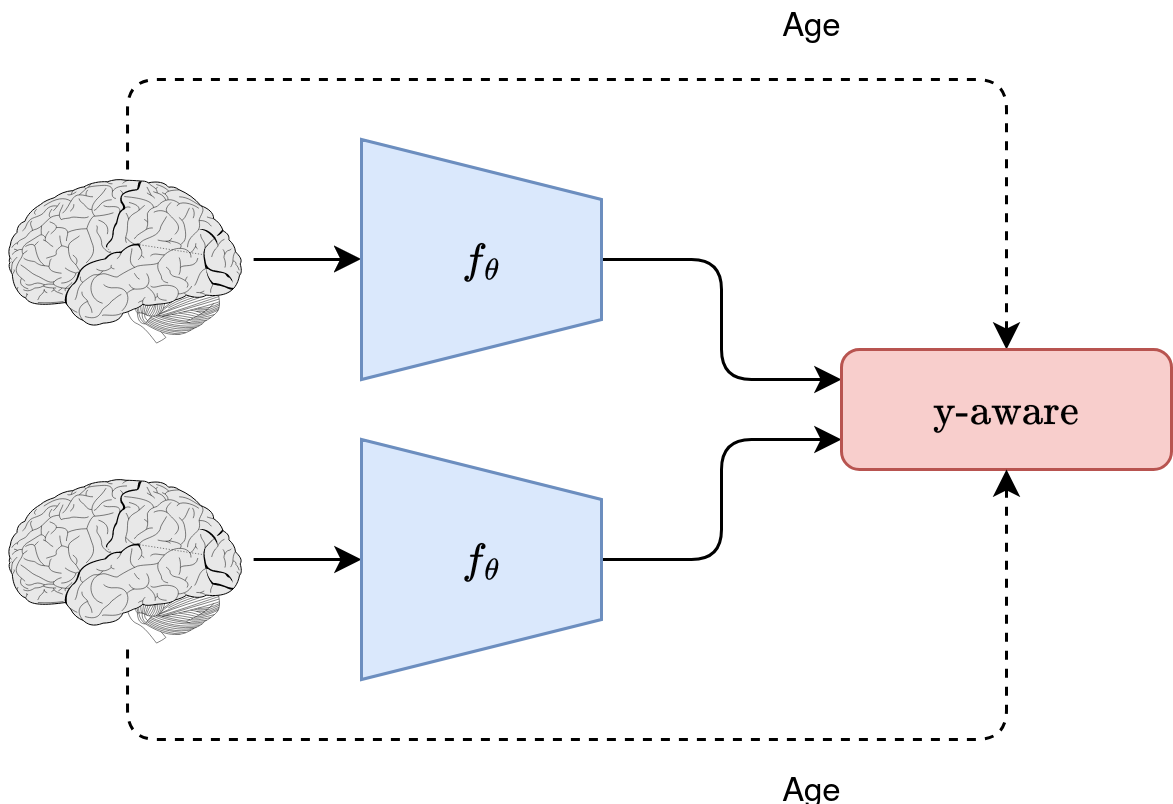
\includegraphics[width=.5\textwidth]{source/yaware_summary.png}
\end{frame}

\begin{frame}{Proposed Approach}
    \centering
    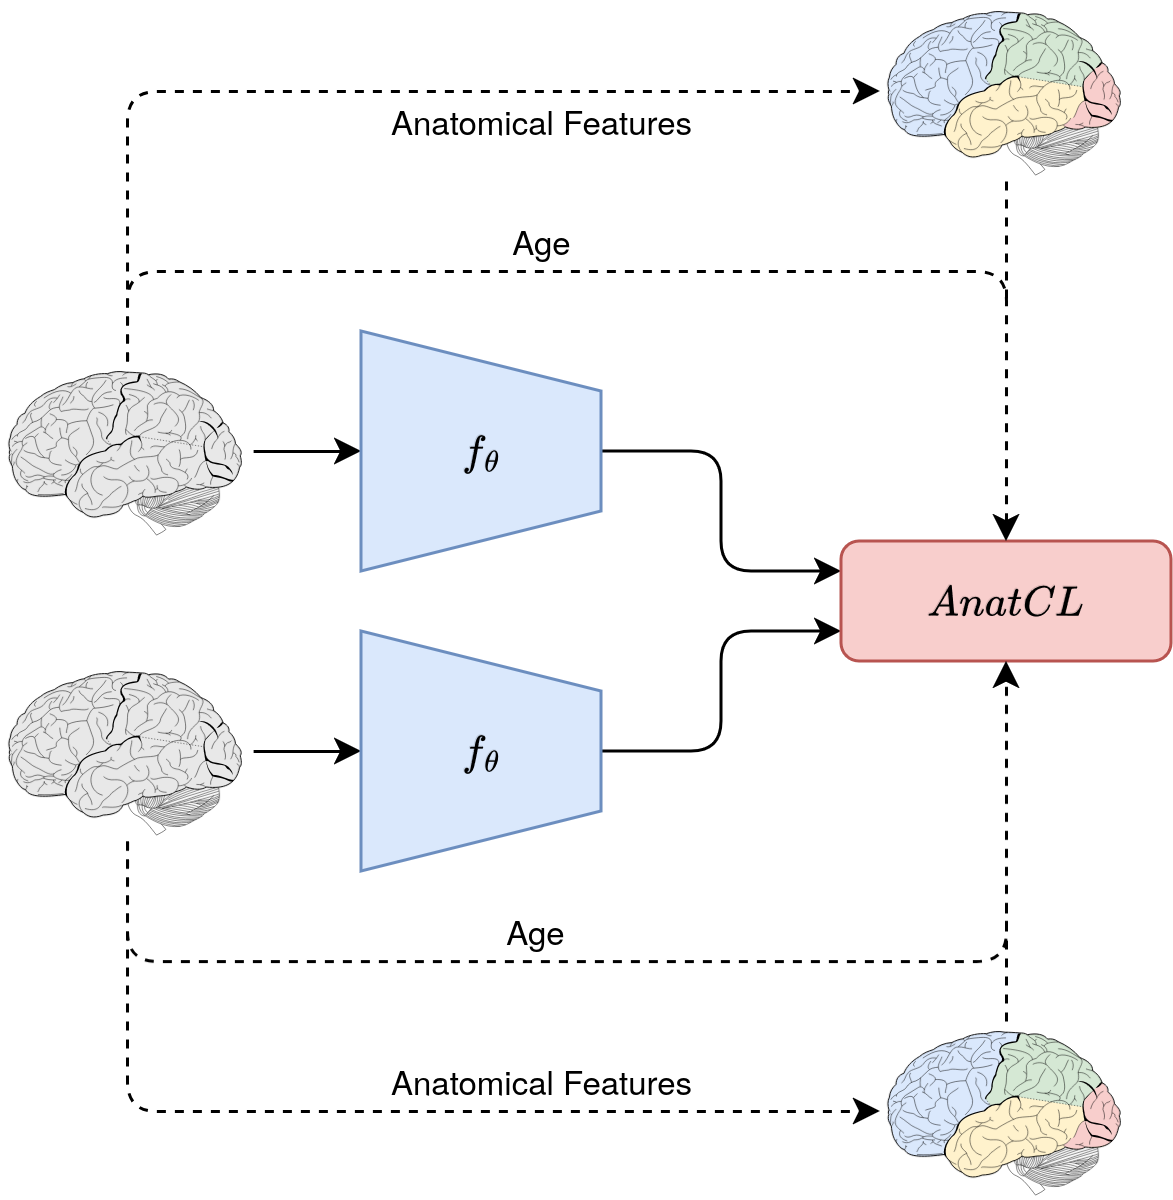
\includegraphics[width=.4\textwidth]{source/anatcl_summary.png}
\end{frame}

% 6


% 5



% 9
\begin{frame}{Integrating Anatomical Information}
\begin{columns}
    \begin{column}{.5\textwidth}
    \begin{itemize}
        \item For each $i^{th}$ patient, its \textbf{anatomical measures} are
        stored in a matrix $\mathcal{D}^i \in \mathbb{R}^{68 \times 7}$
        \item Each \textbf{row vector} contain 7 anatomical measures,
        corresponding to a specific \textbf{region of interest} out of the total
        68
    \end{itemize}
    \begin{center}
        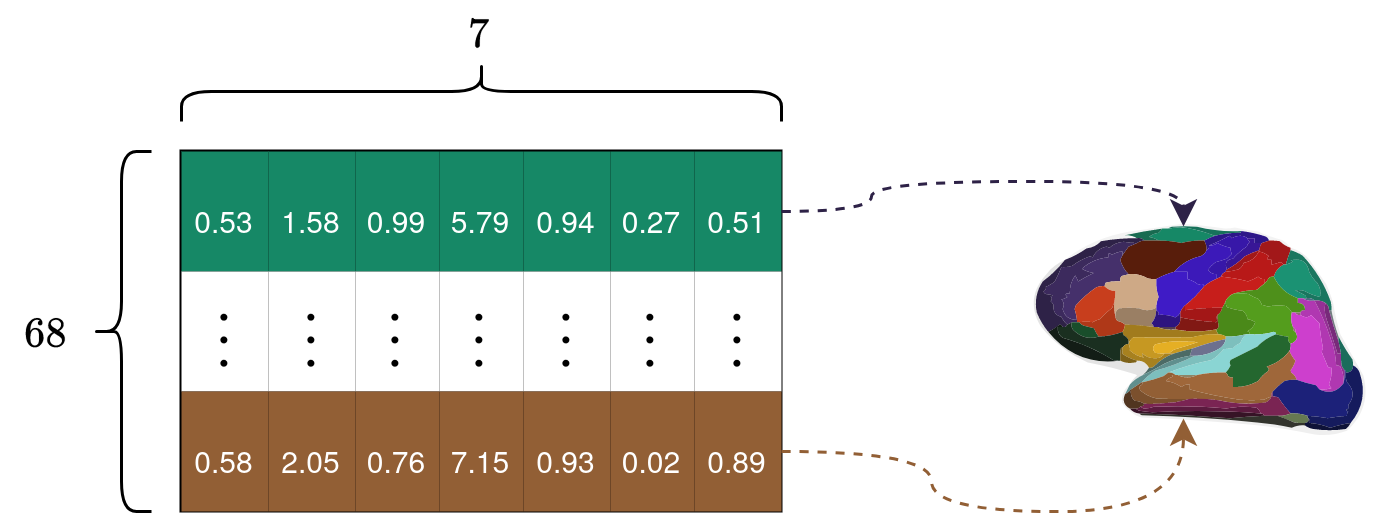
\includegraphics[width=\textwidth]{source/desikan.png}
    \end{center}
    \end{column}
    \begin{column}{.5\textwidth}
        \textbf{Anatomical Measures:}
        \begin{itemize}
            \item Average Cortical Thickness
            \item Standard Deviation Cortical Thickness
            \item Gray Matter Volume
            \item Total Surface Area
            \item Integrated Mean Curvature
            \item Gaussian Curvature
            \item Intrinsic Curvature Index
        \end{itemize}
    \end{column}
\end{columns}
\end{frame}

% 10
\begin{frame}{Proposed Method: Local Descriptor}
\begin{itemize}
    \item Define the \textbf{similarity} between two subjects as the expected
    cross-similarity between local measurements vectors
    \item A \textbf{normalization} $\gamma(\mathbf{x})$ must be applied to
    normalize \textbf{each component} of the vectors to a common range
\end{itemize}
\begin{equation*}
   w_k = \frac{1}{68} \sum^{68}_{n=1} sim(\gamma(\mathcal{D}^i_n), \gamma(\mathcal{D}^k_n)) 
\end{equation*}
\end{frame}

% 11
\begin{frame}{Proposed Method: Global Descriptor}
\begin{itemize}
    \item Rather than viewing the data as 68 measurement vectors one can
    consider the format as 7 \textbf{feature vectors}, each composed of 68
    measurement values 
    \item Let $\omega^i_n = \left( \mathcal{D}^i \right)^T_n$ be the $n^{th}$
    row vector of the \textbf{transposed measurements matrix} associated to the
    $i^{th}$ patient
\end{itemize}
\begin{equation*}
    w_k = \frac{1}{7}\sum_{n=1}^{7} sim(\omega^i_n, \omega^k_n)
\end{equation*}
\end{frame}

\begin{frame}{Descriptors Summary}
\begin{picture}(0, 0)
    \put(260, 25){Local Descriptor}
    \put(-10, 0){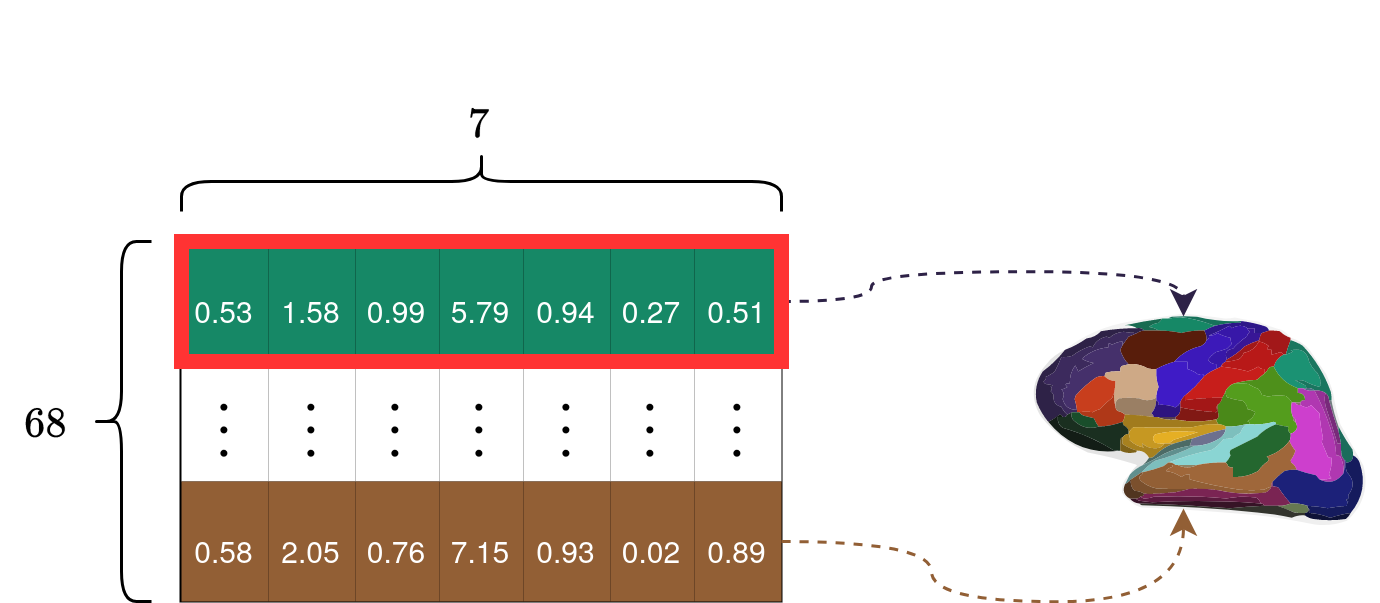
\includegraphics[width=230pt]{source/local_descriptor_summary.png}}
    \put(-10, -90){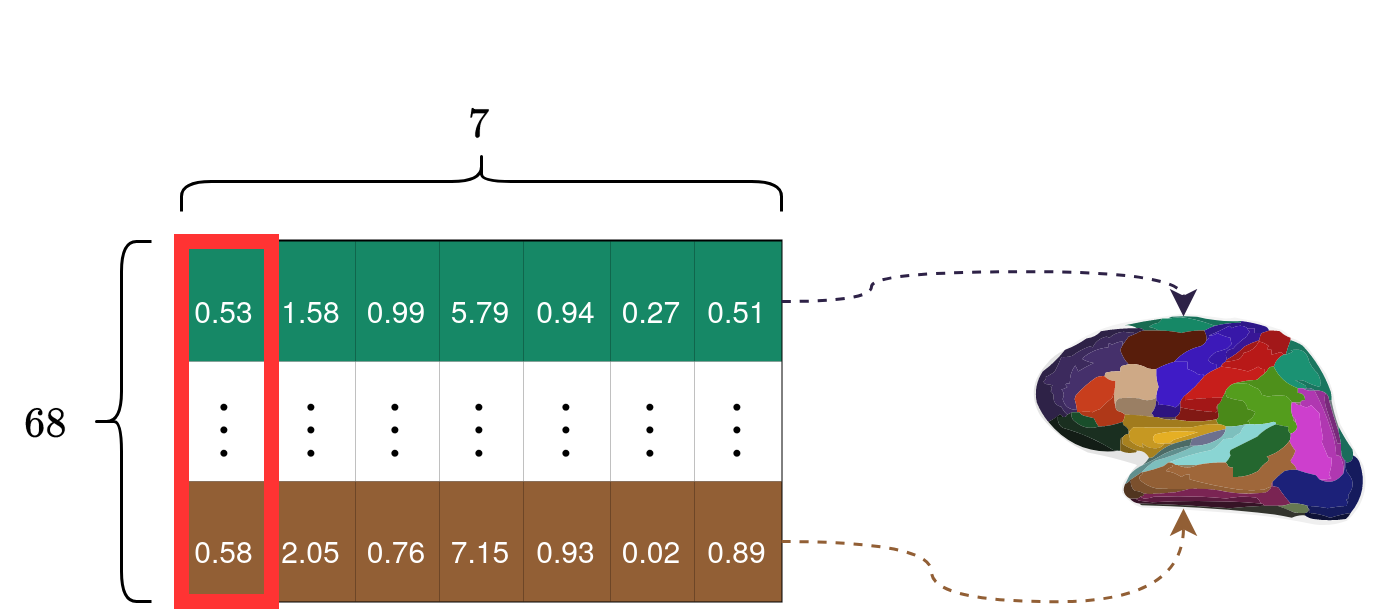
\includegraphics[width=230pt]{source/global_descriptor_summary.png}}
    \put(260, -60){Global Descriptor}
\end{picture}
\end{frame}

% 12
\begin{frame}{Final Formulation}
\begin{itemize}
    \item To incorporate also the age attribute into the final objective loss,
    the resulting function is structured as a \textbf{weighted sum}
    \item This sum combines a weakly supervised loss that is augmented with the
    \textbf{age} attribute ($\mathcal{L}^{\text{age}}$) and another weakly
    supervised loss that utilizes the \textbf{anatomical information}
    ($\mathcal{L}^{\text{AnatCL}}$)
\end{itemize}
\begin{equation*}
   L = \lambda_1 \mathcal{L}^{\text{age}} + \lambda_2\mathcal{L}^{\text{AnatCL}}
\end{equation*}
\end{frame}

\begin{frame}{Experiments Overview}
\begin{itemize}
\item The proposed method was compared with other \textbf{baselines} such as:
\begin{itemize}
    \item \textbf{L1}: Mean Absolute error using the age attribute
    \item \textbf{SimCLR}: Unsupervised Contrastive (\emph{Chen et. al, 2020})
    \item \textbf{y-aware}: Weakly Supervised Contrastive (\emph{Dufumier et. al, 2021})
    \item \textbf{ExpW}: Weakly Supervised Contrastive (\emph{Barbano et. al, 2023})
\end{itemize}
\item The \textbf{experimental setting} consisted in training a ResNet18 model
for each evaluated method on a dataset of \textbf{healthy individuals}
\item Each trained model was then tested on 20 different \textbf{downstream
tasks} across 5 \textbf{different datasets} in a 5 fold cross-validation
\item Experiments were run using the Leonardo CINECA HPC cluster on Nvidia A100
GPUs, with each experiment taking approximately 24 hours
\end{itemize}
    
\end{frame}

% 13
\begin{frame}{Experiments}
% %}
\begin{columns}
    \begin{column}{0.5\textwidth}
        \resizebox{.9\textwidth}{!}{  
        \centering
        \begin{tabular}{l l}
        \toprule
        \textbf{Dataset} & \textbf{Task / Condition} \\
        \midrule
        \textbf{OpenBHB} & Age (HC)   \\
                & Sex   \\
        \midrule
        \textbf{ADNI}    & Alzheimer's Disease \\
                & sMCI vs pMCI \\
        \textbf{OASIS-3} & Alzheimer's Disease \\
        \textbf{SchizConnect} & Schizophrenia Broad \\
                     & Schizophrenia Strict \\
                     & Bipolar Disorder \\
                     & Schizoaffective \\
        \textbf{ABIDE I} & Autism \\
                & Aspergers \\
                & PDD-NOS \\
        \bottomrule
        \end{tabular}
        }
    \end{column}
    \begin{column}{0.5\textwidth}
    \resizebox{.9\textwidth}{!}{
        \centering
        \begin{tabular}{l l}
        \toprule
        \textbf{Dataset} & \textbf{Phenotype}  \\
        \midrule
        \textbf{SchizConnect}  & AIMS Overall Severity  \\
                      & AIMS Upper Body \\
                      & AIMS Lower Body \\
                      & Depression \\
                      & Handedness \\
                      & SAS GAIT \\
        \textbf{ABIDE I} & Handedness \\
                & FIQ (WASI)\\
                & VIQ (WASI) \\
                & PIQ (WASI) \\
        & \\
        & \\
        \bottomrule
        \end{tabular}}
    \end{column}
\end{columns}
\end{frame}

% 14
\begin{frame}{Results}
\begin{columns}
    \begin{picture}(0,0)
       \put(10, 100){Brain Age Prediction} 
    \end{picture}
    \begin{column}{.5\textwidth}
    \resizebox{.9\textwidth}{!}{
        \centering
        \begin{tabular}{l c c}
        \toprule
        \textbf{Method} & \textbf{Age MAE} & \textbf{Sex}  \\
        \midrule
        SimCLR & \result{5.58}{0.53} & \result{76.7}{1.67} \\
        %
        L1 (age sup.) & \result{2.73}{0.14} & \result{76.7}{0.67} \\
        %
        y-Aware & \result{2.66}{0.06} & \result{79.6}{1.13} \\
        %
        ExpW & \result{2.70}{0.06} & \textbf{\result{80.3}{1.7}} \\
        \midrule
        %
        AnatCL-G3 & \textbf{\result{2.61}{0.08}} & \result{78.2}{1.25} \\
        AnatCL-L3 & \result{2.64}{0.07} & \result{78.2}{0.7}\\
        \bottomrule
        \end{tabular}
    }
    \end{column}
    \begin{picture}(0,0)
       \put(10, 100){Clinical Downstream Tasks} 
    \end{picture}
    \begin{column}{.5\textwidth}
        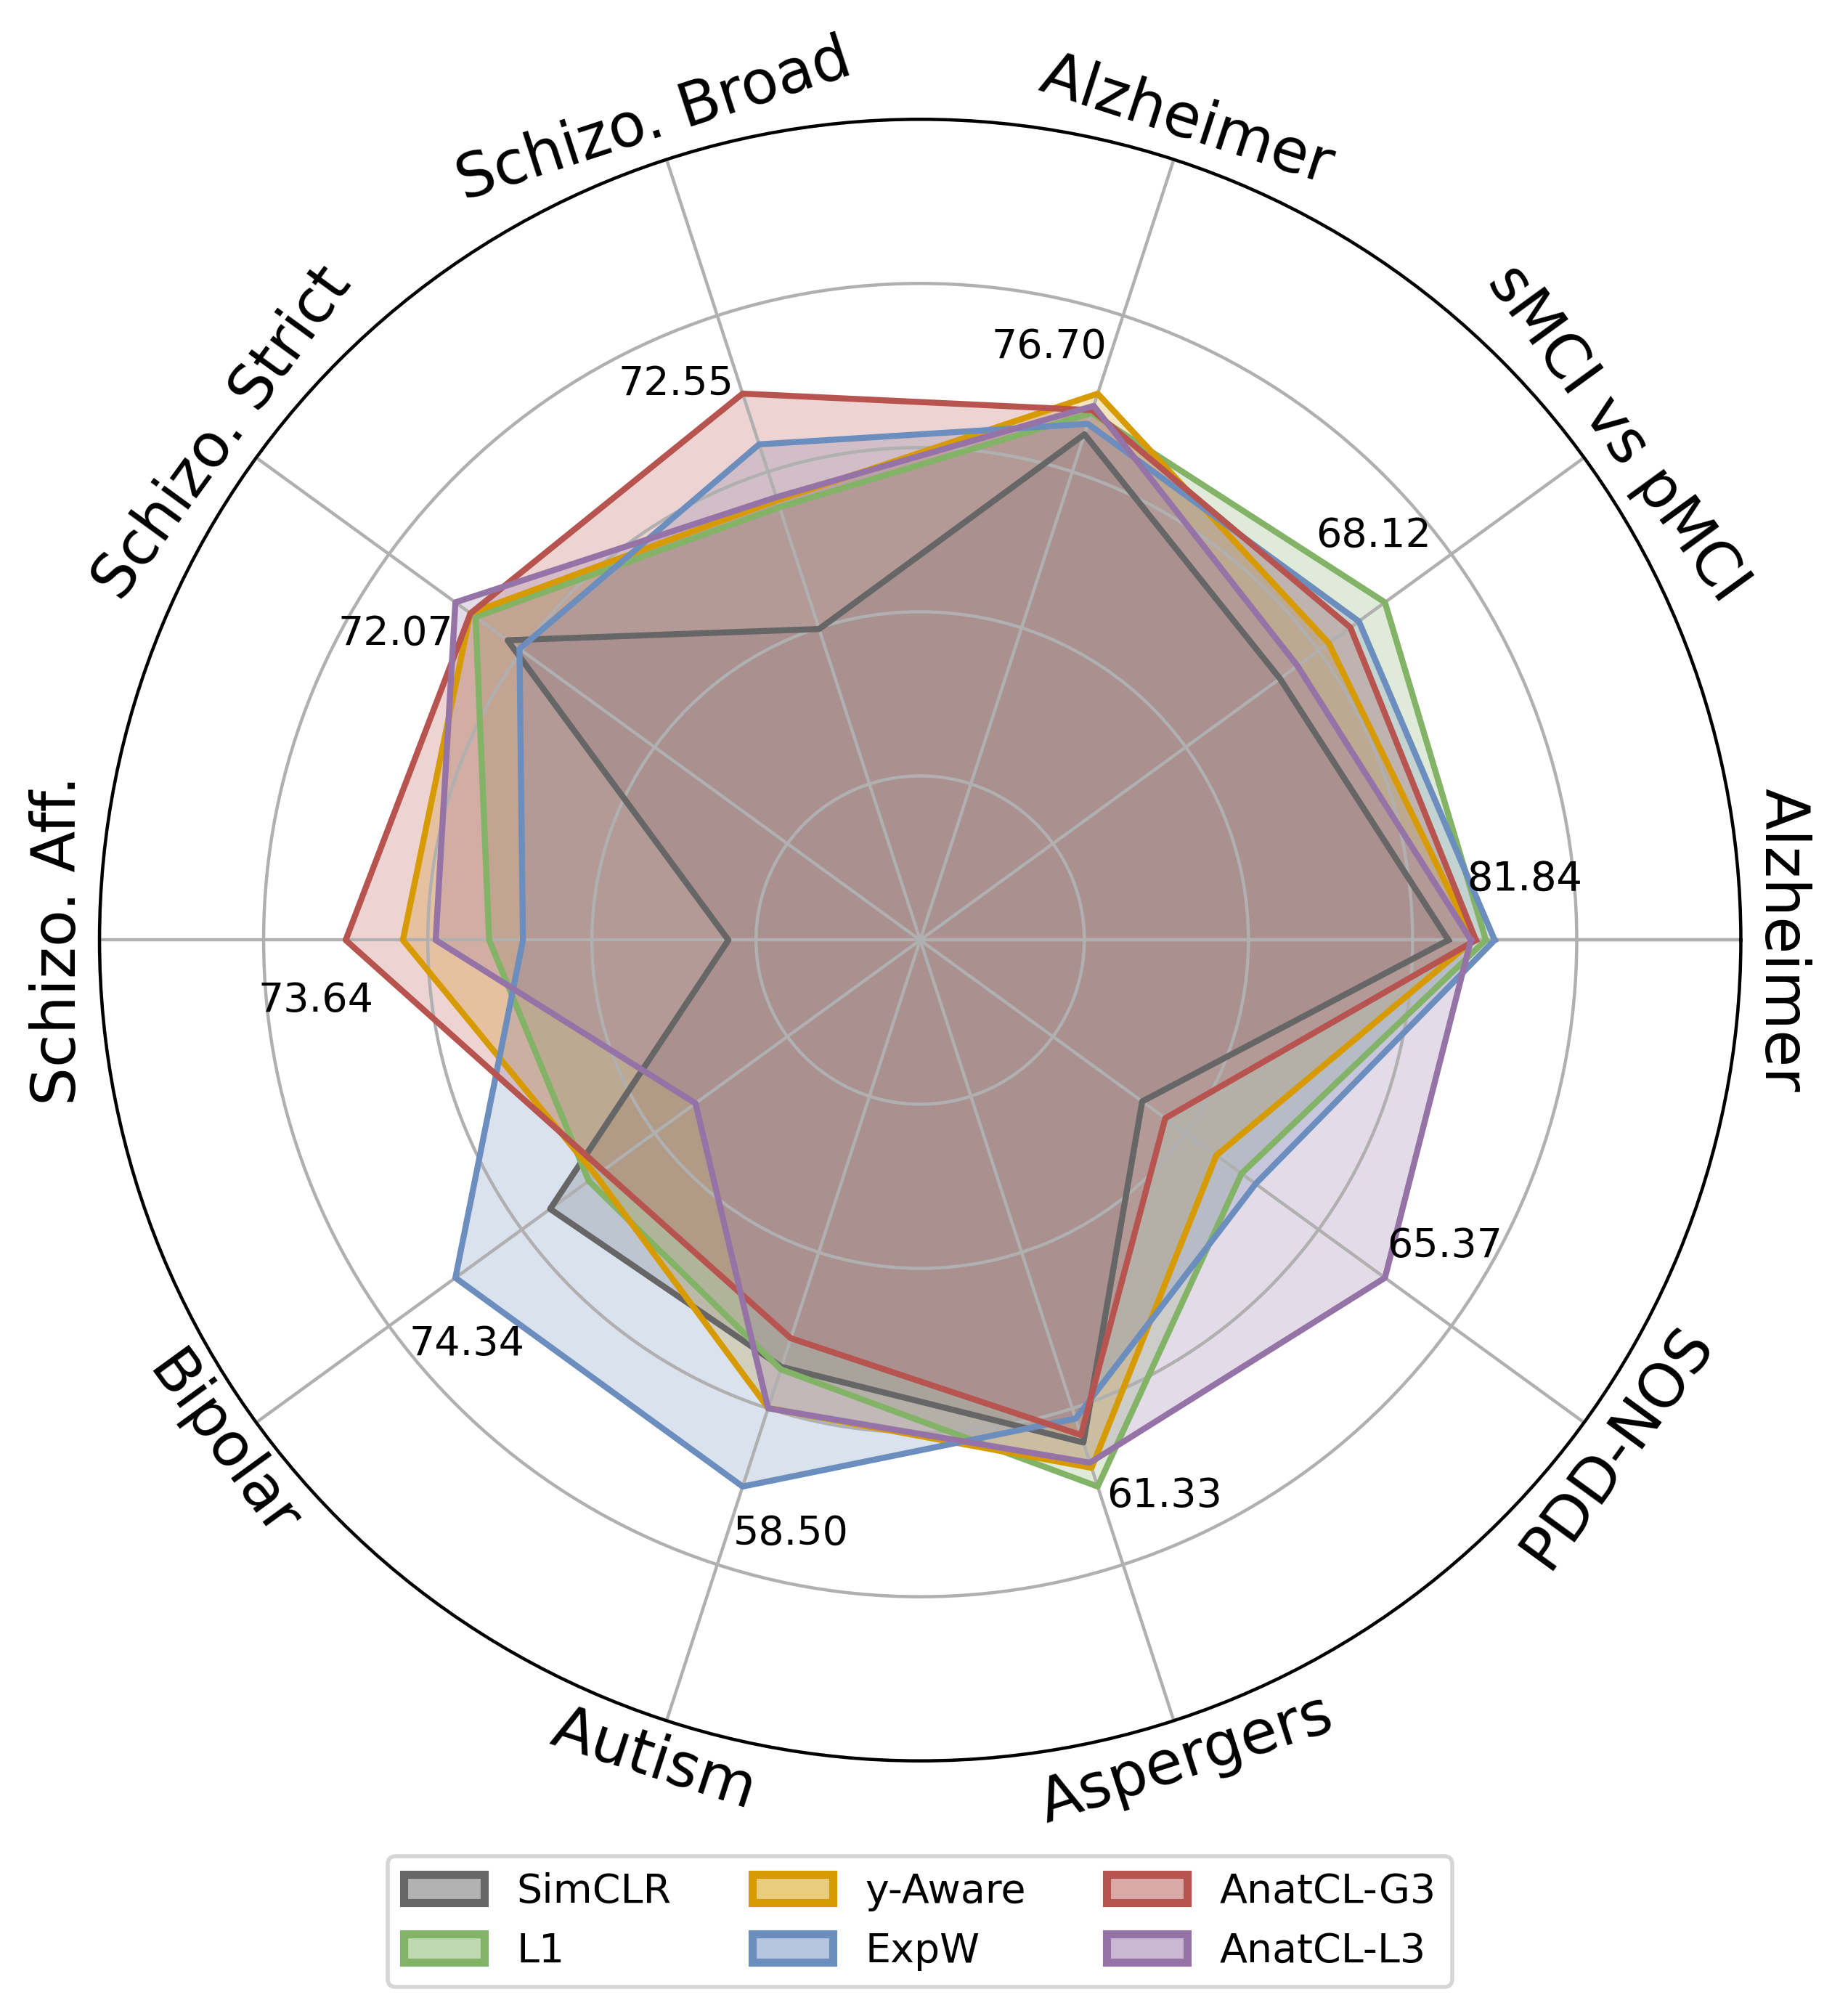
\includegraphics[width=.8\textwidth]{source/polar_plot.png}
    \end{column}
\end{columns}
\end{frame}

% 15
\begin{frame}{Results: Phenotypes and Clinical Scores}
\begin{columns}
    \begin{column}{.5\textwidth}
    \begin{picture}(0, 0)
       \put(10, 10){Abide} 
    \end{picture}
    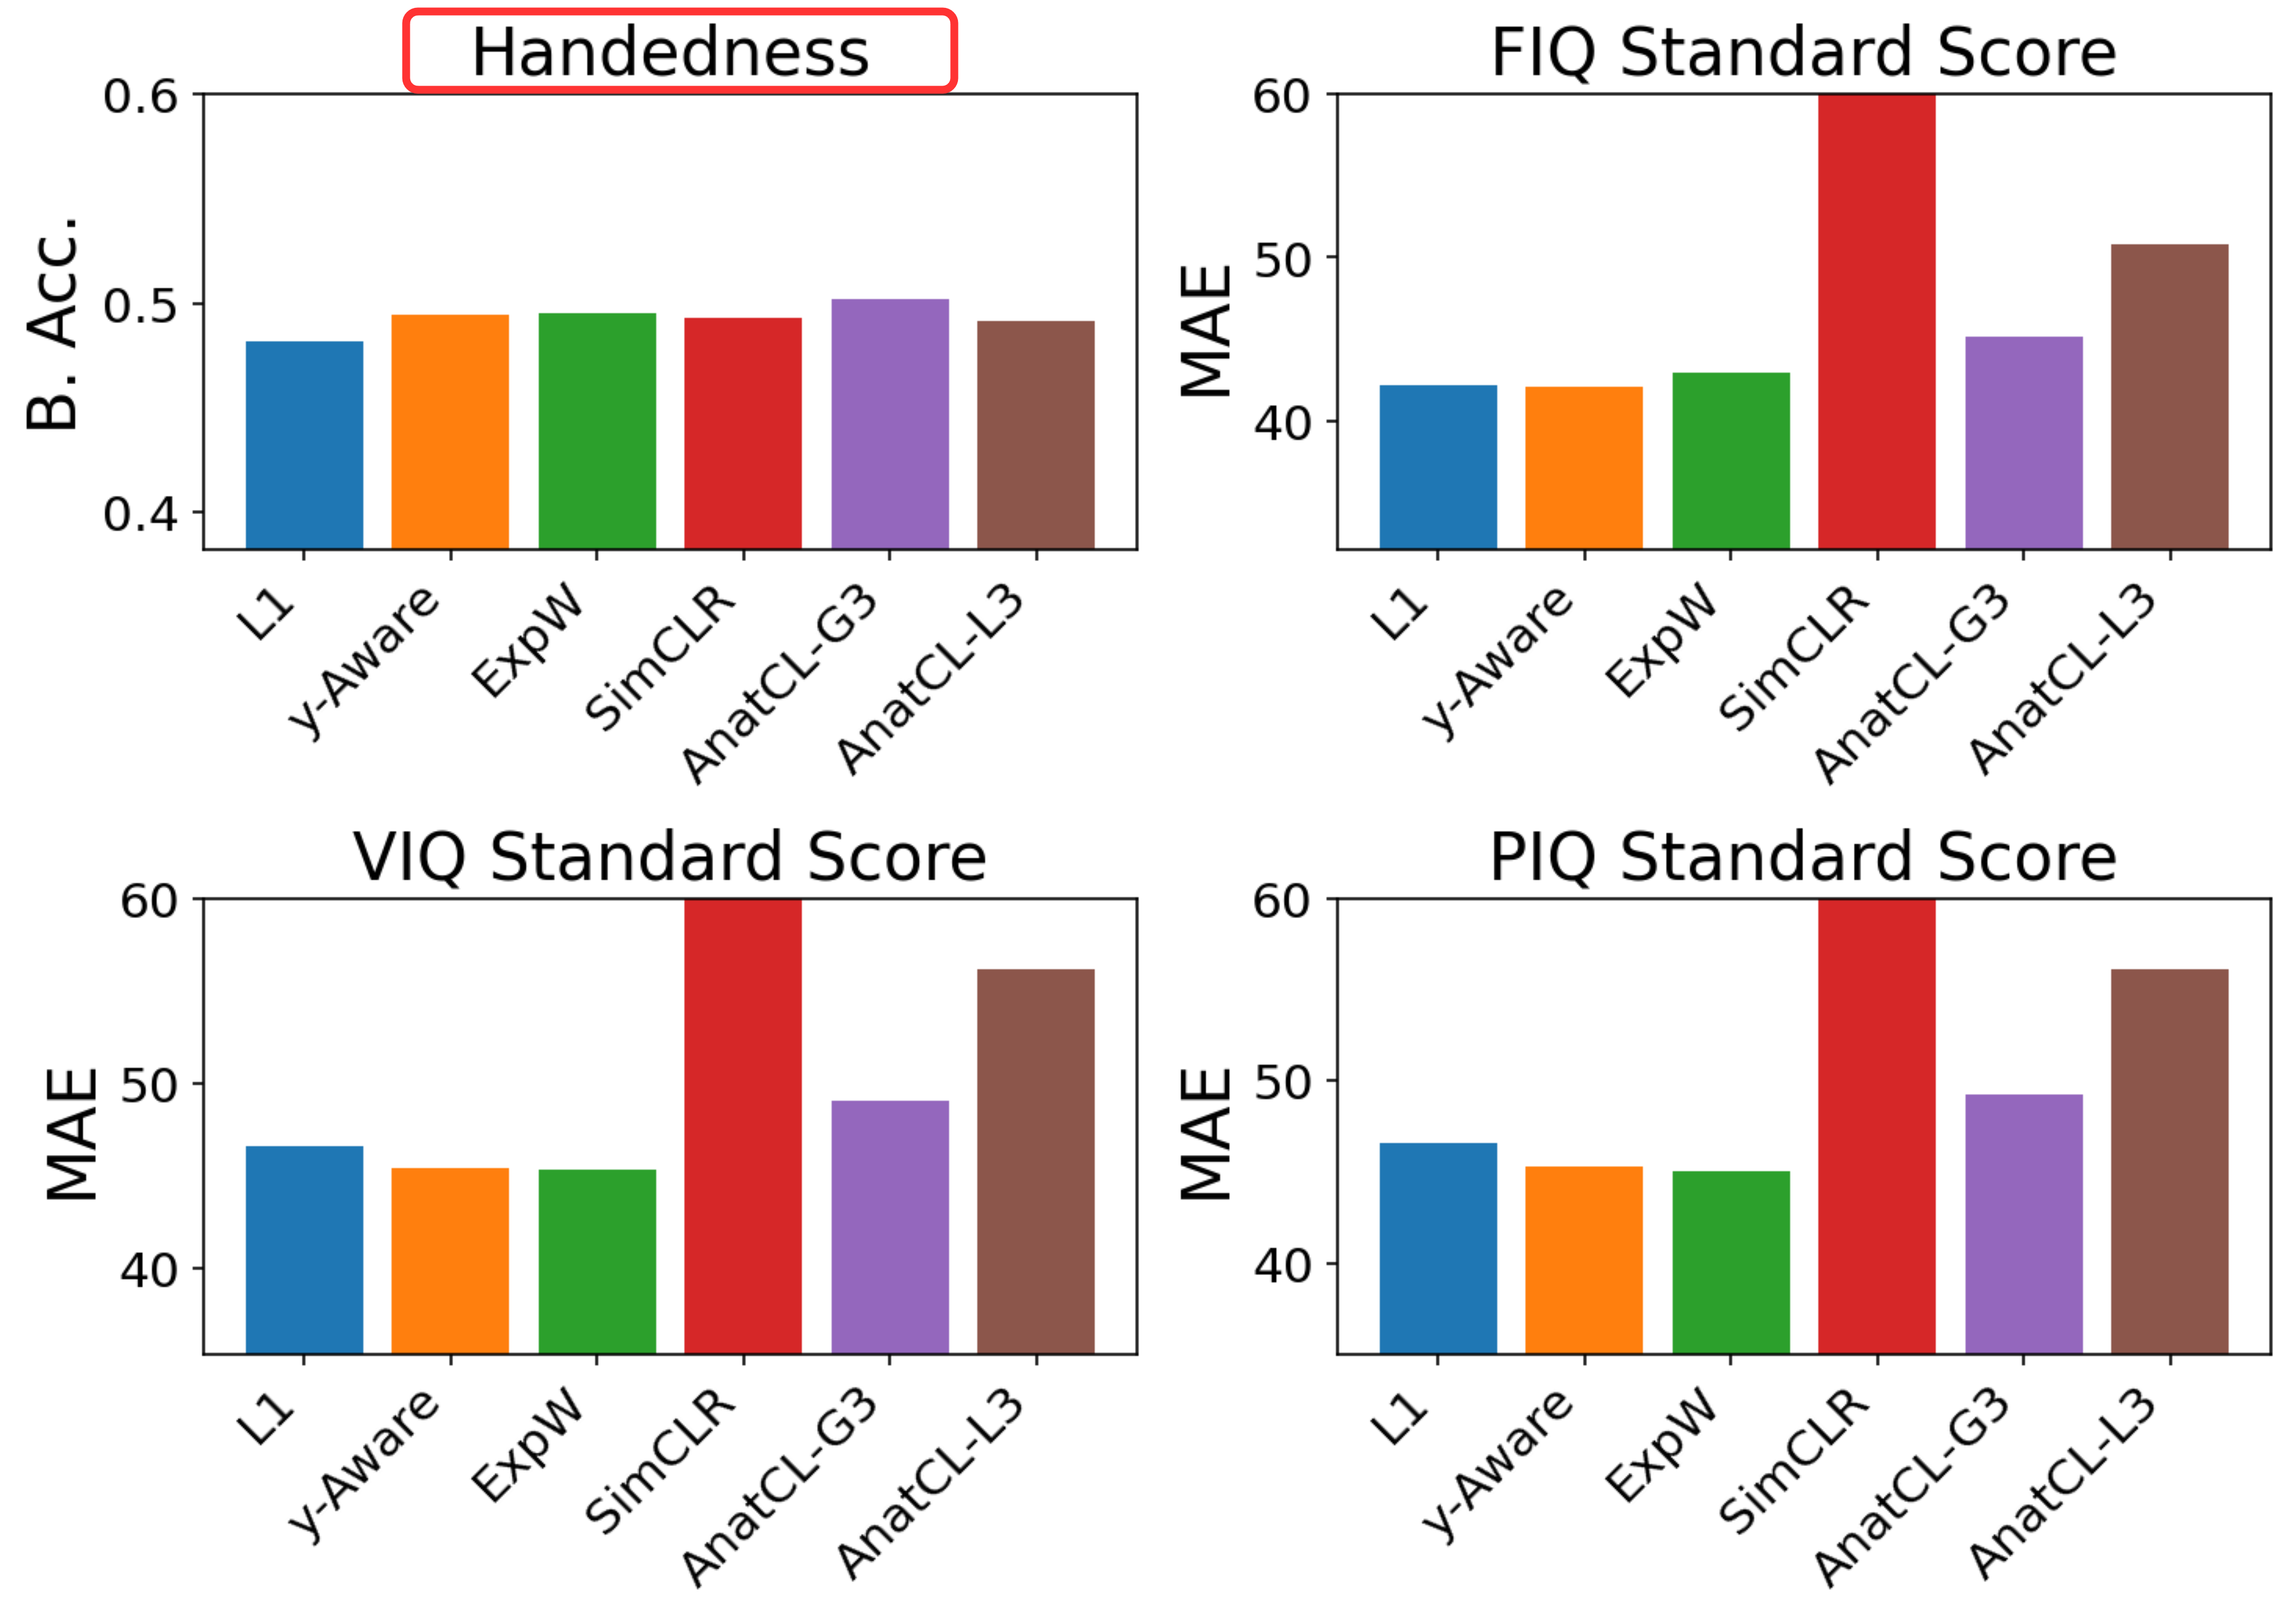
\includegraphics[width=\textwidth]{source/abide_barplot_high.png}
    \end{column}
    \begin{column}{.5\textwidth}
    \begin{picture}(0, 0)
       \put(10, 10){SchizConnect} 
    \end{picture}
    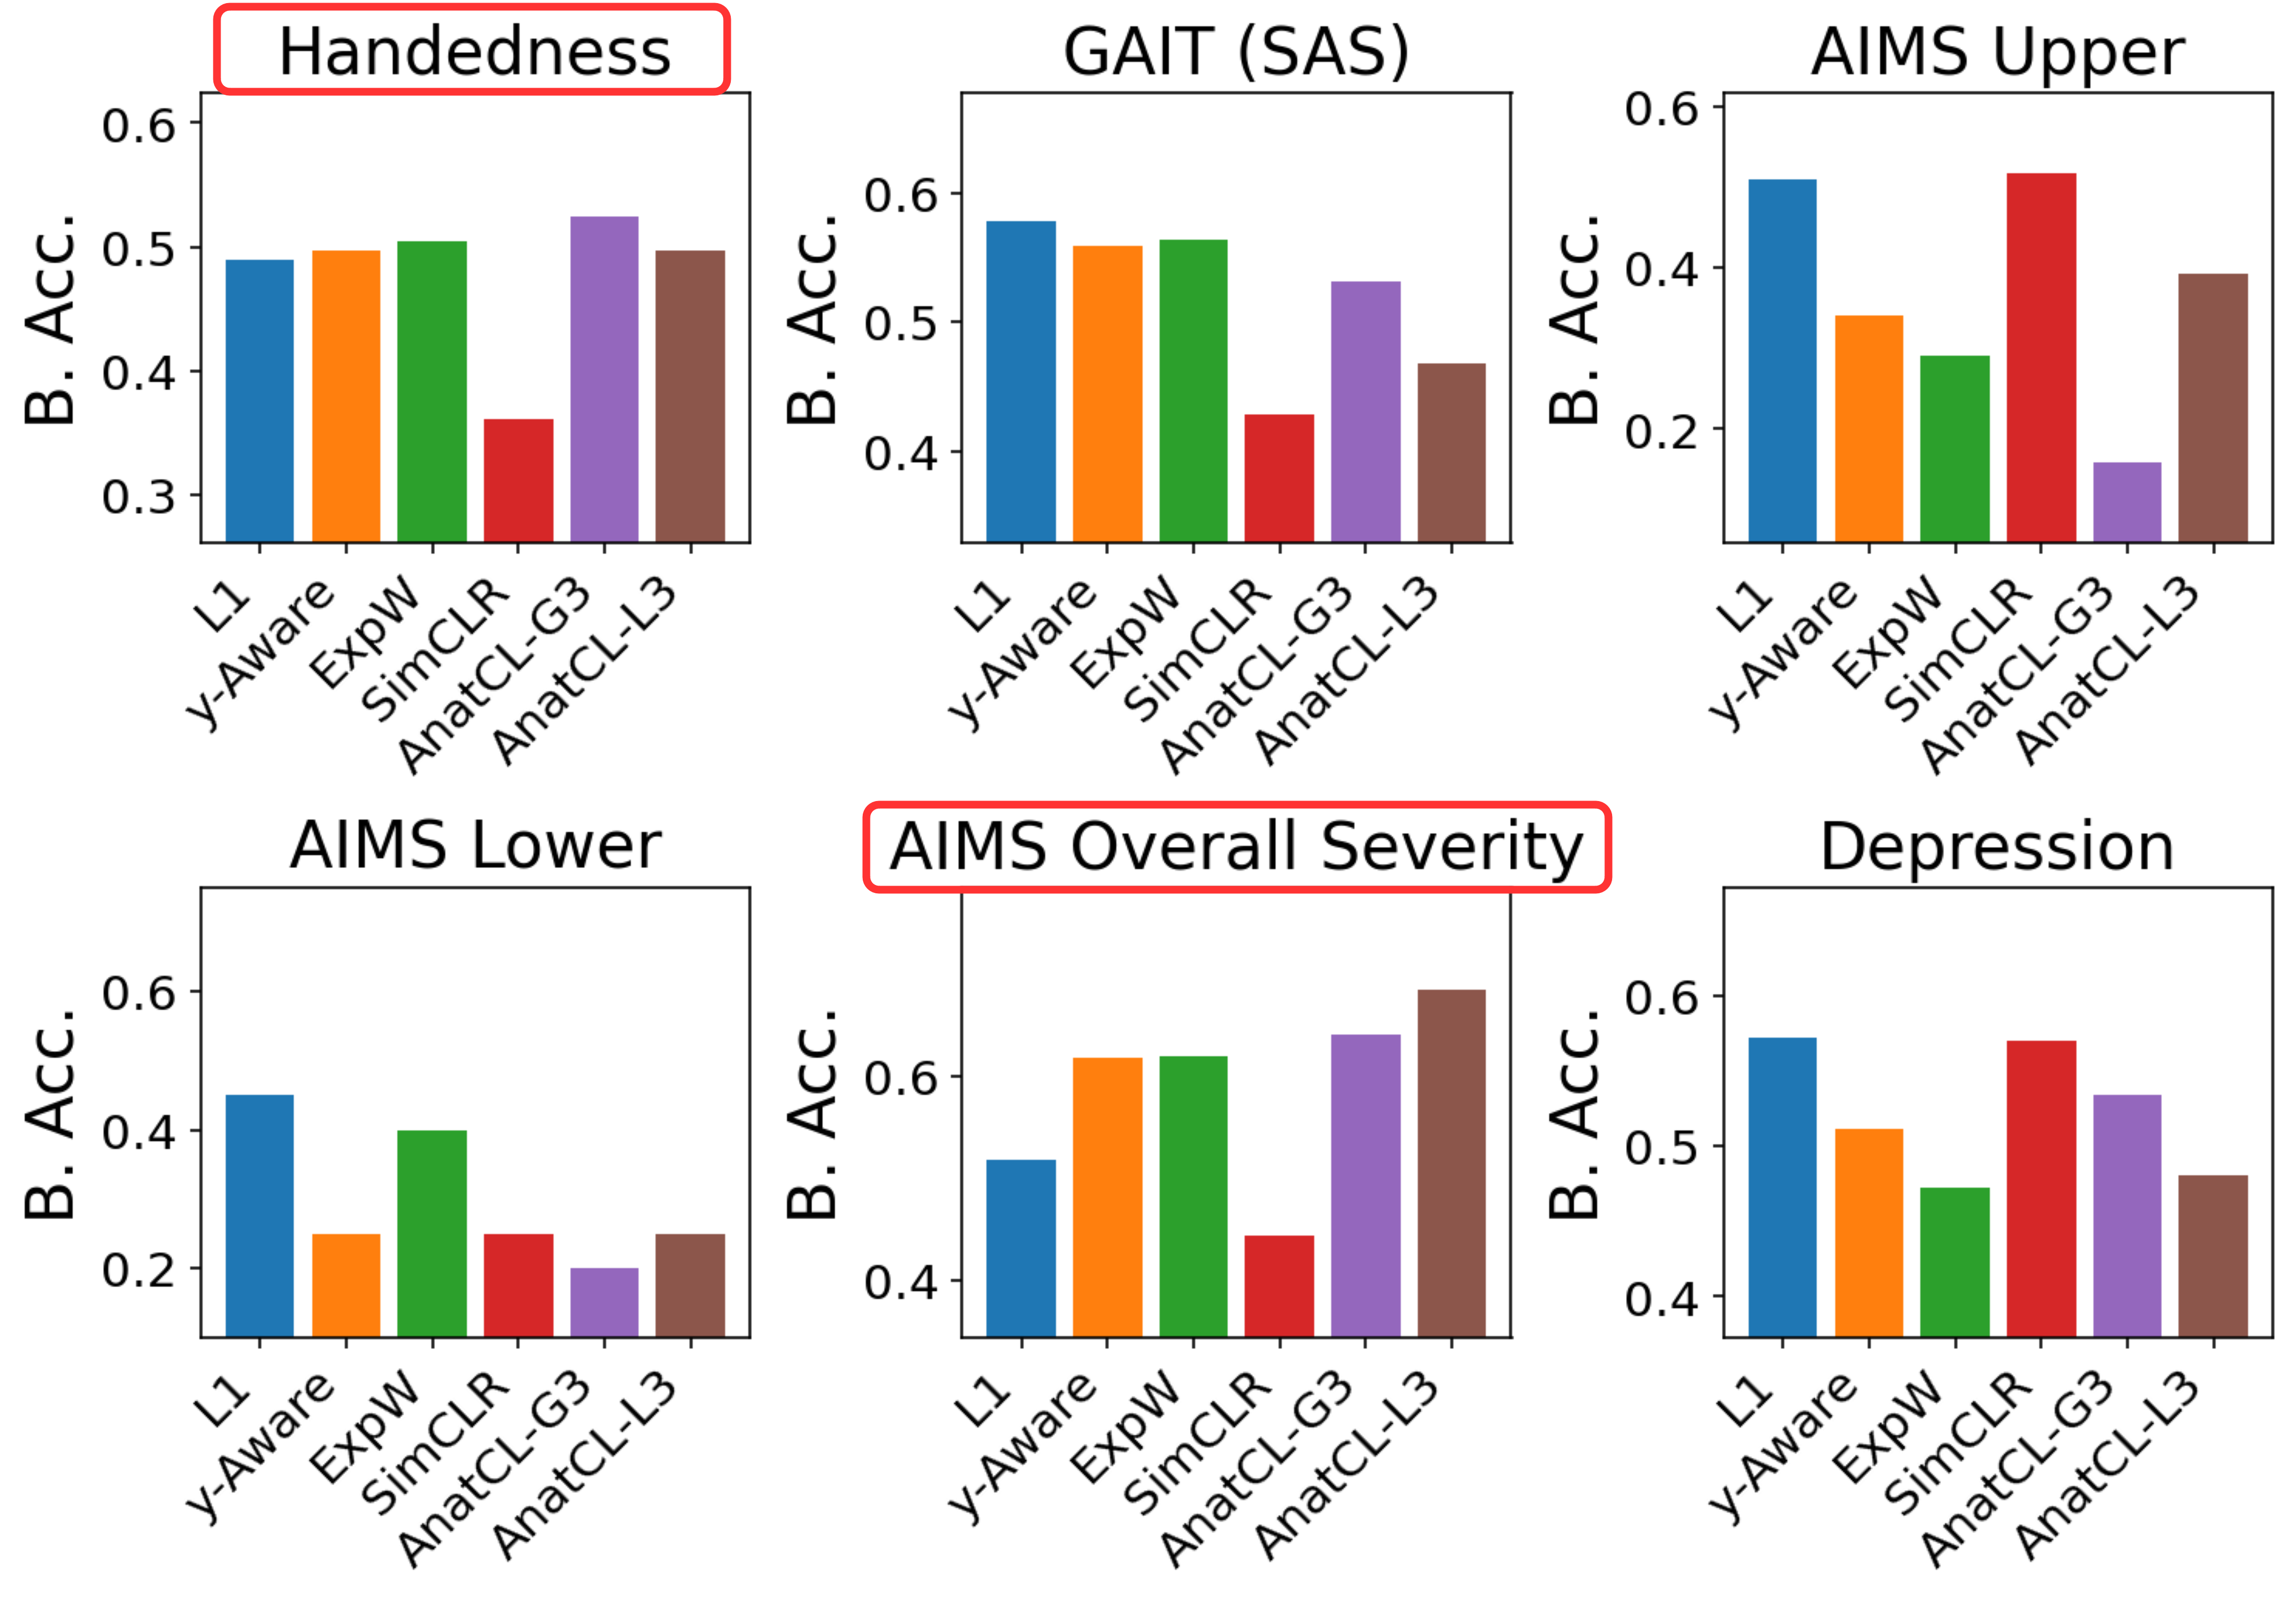
\includegraphics[width=\textwidth]{source/schiz_barplot_high.png}
    \end{column}
\end{columns}
\end{frame}

% 16
\begin{frame}{Conclusions}
\begin{itemize}
    \item The proposed method consistently \textbf{outperforms unsupervised
    methods}, while reaching SOTA performances in some tasks
    \item This suggests that adding anatomical information may actually improve
    the \textbf{generalizability} of the learned representations
    \item This work has been \textbf{submitted} to the NeurIPS conference in May 2024 (\emph{Barbano et. al, Anatomical Foundation Models for Brain MRIs,
    2024})
    \item Further research work is needed to enhance and refine these methods  
\end{itemize}
\end{frame}

% 17
\begin{frame}{Limitations and Future Developments}
\begin{itemize}
    \item The age attribute \textbf{may not} be always present in every
    neuroimaging dataset
    \item Novel methods may integrate \textbf{only} anatomical measures without
    using the age. Those measures can be obtained from pre-processing pipelines
    common in neuroimaging, effectively making the methods fully unsupervised
    \item Additional methods to integrate \textbf{other anatomical measures} can
    be explored
    \item Develop \textbf{multi-modal models} to integrate other
    \textbf{acquisition methods} as well as data of different nature such as
    \textbf{textual data} coming from clinical records/assessments  
\end{itemize}
\end{frame}

% 18
\begin{frame}
\centering
\Huge{\textbf{Thanks for your attention}}\\
\vspace{15pt}
\Large{\emph{Any questions?}}
\end{frame}

\end{document}
